\documentclass{standalone}
\usepackage{tikz}
\usetikzlibrary{decorations.pathreplacing}

\begin{document}
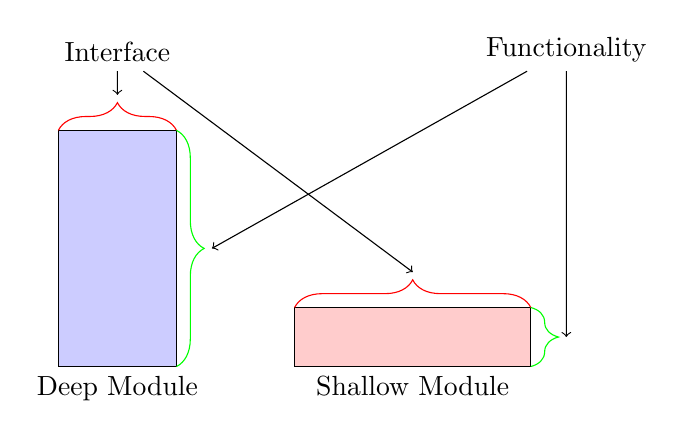
\begin{tikzpicture}[scale = 1.5]
    % 绘制Deep Module并染色
    \draw[fill=blue!20] (0,0) rectangle (1,2);
    \node[below] at (0.5, 0) {Deep Module};
    % 绘制Deep Module上方花括号并染色
    \draw[decorate, decoration={brace, amplitude=10pt}, red] (0,2) -- (1,2);
    % 标记Deep Module上方花括号线条中点
    \coordinate (deep_brace_top_mid) at (0.5, 2 + 0.3);

    % 绘制Deep Module右侧花括号并染色
    \draw[decorate, decoration={brace, amplitude=10pt, mirror}, green] (1,0) -- (1,2);
    % 标记Deep Module右侧花括号线条中点
    \coordinate (deep_brace_right_mid) at (1 + 0.3, 1);

    % 绘制Shallow Module并染色
    \draw[fill=red!20] (2,0) rectangle (4, 0.5);
    \node[below] at (3,0) {Shallow Module};
    % 绘制Shallow Module上方花括号并染色
    \draw[decorate, decoration={brace, amplitude=10pt}, red] (2,0.5) -- (4,0.5);
    % 标记Shallow Module上方花括号线条中点
    \coordinate (shallow_brace_top_mid) at (3, 0.5 + 0.3);

    % 绘制Shallow Module右侧花括号并染色
    \draw[decorate, decoration={brace, amplitude=10pt, mirror}, green] (4,0) -- (4,0.5);
    % 标记Shallow Module右侧花括号线条中点
    \coordinate (shallow_brace_right_mid) at (4 + 0.3, 0.25);

    \node[above] at (0.5,2.5) (interface) {Interface};
    \node[above] at (4.3, 2.5) (functionality) {Functionality};

    % 绘制从 Interface 指向两个上方 brace decorate 的线条
    \draw[->] (interface) -- (deep_brace_top_mid);
    \draw[->] (interface) -- (shallow_brace_top_mid);

    % 绘制从 Functionality 指向新增两个 brace decorate 的线条
    \draw[->] (functionality) -- (deep_brace_right_mid);
    \draw[->] (functionality) -- (shallow_brace_right_mid);
\end{tikzpicture}
\end{document}
